% Источник: lectures_01_[04.09.2026].tex 15–34, 60–70, 223–227; lectures_08_10_sets.tex 26–52; lecture_09_probability.tex 3–15.
\question{Случайный эксперимент и вероятностное пространство}

\begin{definition}[\topicmark{Случайный эксперимент}Случайный эксперимент]
Случайный эксперимент — процесс, наблюдение или действие, результат которого невозможно точно предсказать заранее. К нему предъявляются три требования.
\begin{enumerate}
\item \textbf{Отсутствие детерминированной регулярности.} При повторении в неизменных условиях результаты могут различаться.
\item \textbf{Воспроизводимость.} Опыт можно многократно повторить в одних и тех же контролируемых условиях.
\item \textbf{Статистическая устойчивость.} При большом числе повторений относительная частота исхода стабилизируется.
\end{enumerate}
\end{definition}

\begin{definition}[\topicmark{Вероятностное пространство}Вероятностное пространство]
Вероятностное пространство — тройка $(\Omega,\mathcal F,\Pr)$.

\smallskip
Множество $\Omega$ состоит из элементарных исходов $\omega$, $\mathcal F$ — $\sigma$-алгебра событий, а $\Pr\colon\mathcal F\to[0;1]$ — $\sigma$-аддитивная мера с $\Pr(\Omega)=1$.
\end{definition}

\begin{definition}[\topicmark{Сигма-алгебра}$\sigma$-алгебра]
Семейство подмножеств $\mathcal F\subseteq 2^\Omega$ называется
\textbf{$\sigma$-алгеброй} на $\Omega$, если выполнены три условия.
\begin{enumerate}[label=\arabic*)]
\item $\Omega\in\mathcal F$.
\item Если $A,B\in\mathcal F$, то их пересечение $A\cap B$, объединение
      $A\cup B$, разность $A\setminus B$ и симметрическая разность
      $A\triangle B$ тоже принадлежат $\mathcal F$.
\item Если $A_1,A_2,\ldots\in\mathcal F$, то их счётное объединение
      $\bigcup_{i=1}^{\infty}A_i$ принадлежит $\mathcal F$.
\end{enumerate}
\end{definition}

\begin{definition}[\topicmark{Сигма-аддитивность}$\sigma$-аддитивность]
    Мера $\Pr$ называется \textbf{$\sigma$-аддитивной}, если
    для попарно непересекающихся $A_i\in\mathcal{F}$
    \[
        \Pr\left(\bigsqcup_{i=1}^{\infty}A_i\right)
        =\sum_{i=1}^{\infty}\Pr(A_i).
    \]
\end{definition}

% Источник: lectures_01_[04.09.2026].tex 243–286.
\question{Дискретное вероятностное пространство. Классическая модель}

% Тервер(Лекция)69.pdf, с. 1: не более чем счётное пространство, все подмножества, поточечная мера.
\begin{definition}[\topicmark{Поточечное задание}Дискретное вероятностное пространство]
Множество исходов $\Omega$ конечно или счётно, а $\mathcal F=2^\Omega$.
Каждому исходу $\omega$ приписывают число $p_\omega\geq0$, причём
$\sum_{\omega\in\Omega}p_\omega=1$. Эти числа задают вероятность любого события:
\[
  \Pr(A)=\sum_{\omega\in A}p_\omega,\qquad
  p_\omega=\Pr(\{\omega\}).
\]
\end{definition}

\begin{theorem}[\topicmark{Классическая вероятность}Формула классической вероятности]
В классической модели все элементарные исходы равновероятны. Для события $A$ выполняется $\Pr(A)=|A|/|\Omega|$.
\end{theorem}
\begin{Proof}
Обозначим вероятность каждого исхода через $c$. Из нормировки
\[
1=\Pr(\Omega)=\sum_{\omega\in\Omega}\Pr(\{\omega\})=|\Omega|c
\]
получаем $c=1/|\Omega|$. Складывая вероятности исходов из $A$, находим
\[
 \Pr(A)=\sum_{\omega\in A}\frac1{|\Omega|}=\frac{|A|}{|\Omega|}.
\]
\end{Proof}

% Источник: lectures_01_[04.09.2026].tex 301–359; lectures_02_[11.09.2026].tex 546–558.
\question{Урновая схема с возвращением. Испытания Бернулли}

\begin{task}[\topicmark{Выбор с возвращением}Выбор с возвращением]
Из урны, содержащей $M$ красных и $N-M$ чёрных шаров, $n$ раз наугад извлекают шар и возвращают его. Найти вероятность события $A$: среди извлечённых шаров ровно $k$ красных.
\end{task}
\begin{solution}
Пронумеруем шары от $1$ до $N$, начиная с красных. Исход — упорядоченная последовательность номеров. При каждом выборе доступны все $N$ шаров, поэтому всего $N^n$ равновероятных исходов.

\smallskip
Для события $A$ выбираем $k$ позиций красных шаров из $n$. На каждой из этих позиций номер выбирается $M$ способами, на каждой из остальных — $N-M$ способами. Получаем
\[
 |A|=C_n^k M^k(N-M)^{n-k},\qquad
 \Pr(A)=\frac{|A|}{N^n}=C_n^k p^k(1-p)^{n-k},\quad p=\frac MN.
\]
\end{solution}

\begin{definition}[\topicmark{Испытания Бернулли}Схема испытаний Бернулли]
Проводятся $n$ независимых испытаний с двумя исходами и постоянной вероятностью успеха $p$.

\smallskip
Для конкретной последовательности $(i_1,\ldots,i_n)$ из нулей и единиц, содержащей $k=\sum_{j=1}^n i_j$ успехов, вероятность равна $p^k(1-p)^{n-k}$.
\end{definition}
В урновой схеме успех — выбор красного шара. Возвращение и перемешивание восстанавливают состав урны перед каждым новым выбором. Испытания независимы, и вероятность успеха при каждом выборе равна $M/N$.

% Источник: lectures_01_[04.09.2026].tex 387–399; lectures_02_[11.09.2026].tex 1–55.
\question{Геометрическая вероятность. Задача о встрече}

\begin{definition}[\topicmark{Геометрическая вероятность}Геометрическая вероятность]
При равномерном выборе точки из области $\Omega$ вероятность попадания в измеримое множество $A$ равна $\lambda(A)/\lambda(\Omega)$, где $\lambda$ — длина, площадь или объём.

\smallskip
Например, на $[0;1]$ имеем $\Pr(A)=\lambda(A)$.
\end{definition}

\begin{example}[\topicmark{Задача о встрече}Задача о встрече]
    Два человека независимо и равномерно выбирают время прихода
    с 12:00 до 13:00. Каждый ждёт другого не более 20 минут.
    Найти вероятность встречи.

    \smallskip
    \textbf{Решение.}
    Пусть $x$ и $y$ --- время прихода в минутах после 12:00.
    Тогда
    \[
        \Omega = [0; 60] \times [0; 60].
    \]
    Событие встречи:
    \[
        \mathcal{A}
        = \{(x,y) \in \Omega \colon |x-y| \leq 20\}.
    \]

    \begin{center}
        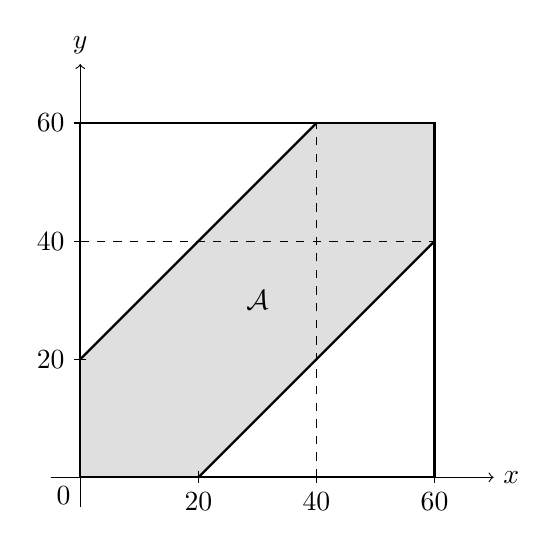
\begin{tikzpicture}[x=0.075cm, y=0.075cm]
            \fill[gray!25]
                (0,0) -- (20,0) -- (60,40) --
                (60,60) -- (40,60) -- (0,20) -- cycle;

            \draw[thick] (0,0) rectangle (60,60);
            \draw[thick] (0,20) -- (40,60);
            \draw[thick] (20,0) -- (60,40);

            \draw[dashed] (0,40) -- (60,40);
            \draw[dashed] (40,0) -- (40,60);

            \draw[->] (-5,0) -- (70,0) node[right] {$x$};
            \draw[->] (0,-5) -- (0,70) node[above] {$y$};

            \node[below left] at (0,0) {$0$};
            \foreach \t in {20,40,60} {
                \draw (\t,1) -- (\t,-1) node[below] {$\t$};
                \draw (1,\t) -- (-1,\t) node[left] {$\t$};
            }

            \node at (30,30) {$\mathcal{A}$};
        \end{tikzpicture}
    \end{center}

    \[
        \Pr(\mathcal{A})
        = \frac{S(\mathcal{A})}{S(\Omega)}
        = \frac{60^2 - 2 \cdot \frac{40^2}{2}}{3600}
        = \frac{2000}{3600}
        = \frac{5}{9}.
    \]
\end{example}

% Источник: lectures_02_[11.09.2026].tex 87–119.
\question{Условная вероятность}

\begin{definition}[\topicmark{Определение}Определение]
    Пусть $\mathcal{A}, \mathcal{B} \in \mathcal{F}$
    и $\Pr(\mathcal{B}) \neq 0$.
    Условной вероятностью события $\mathcal{A}$
    при условии события $\mathcal{B}$ называется число
    \[
        \Pr(\mathcal{A} \mid \mathcal{B})
        =
        \frac{\Pr(\mathcal{A} \cap \mathcal{B})}{\Pr(\mathcal{B})}.
    \]
\end{definition}

\begin{Proof}[\topicmark{Обоснование в классической модели}Обоснование в классической модели]

Пусть $\Pr(\mathcal{B}) > 0$. Если известно, что событие
$\mathcal{B}$ произошло, то остаются только исходы из
$\mathcal{B}$, которые по-прежнему равновероятны.

\smallskip
Из них событию $\mathcal{A}$ благоприятствуют исходы
из $\mathcal{A} \cap \mathcal{B}$. Поэтому
\[
    \Pr(\mathcal{A} \mid \mathcal{B})
    =
    \frac{|\mathcal{A} \cap \mathcal{B}|}{|\mathcal{B}|}
    =
    \frac{
        |\mathcal{A} \cap \mathcal{B}| / |\Omega|
    }{
        |\mathcal{B}| / |\Omega|
    }
    =
    \frac{\Pr(\mathcal{A} \cap \mathcal{B})}{\Pr(\mathcal{B})}.
\]
\end{Proof}

% Источник: lectures_02_[11.09.2026].tex 190–207, 273–316, 319–346.
\question{Формулы полной вероятности, умножения вероятностей и Байеса}

\begin{theorem}[\topicmark{Полная вероятность}Формула полной вероятности]
Пусть события $A_i$ образуют конечное или счётное разбиение $\Omega$ и $\Pr(A_i)>0$. Для каждого события $B$ имеем
\[
 \Pr(B)=\sum_i \Pr(B\mid A_i)\Pr(A_i).
\]
\end{theorem}
% Разложение по разбиению: Тервер(Лекция)68.pdf, с. 5.
% Замена вероятности пересечения: lectures_02_[11.09.2026].tex, строки 273–282.
\begin{Proof}
События $B\cap A_i$ попарно несовместны и в объединении дают $B$.
По счётной аддитивности и по формуле $\Pr(A_i\cap B)=\Pr(A_i)\Pr(B\mid A_i)$
\[
  \Pr(B)=\sum_i\Pr(B\cap A_i)=\sum_i\Pr(B\mid A_i)\Pr(A_i).
\]
\end{Proof}

\begin{theorem}[\topicmark{Умножение вероятностей}Формула умножения вероятностей]
Пусть $\Pr(A_1\cap\cdots\cap A_{n-1})>0$. Тогда
\[
 \Pr(A_1\cap\cdots\cap A_n)
 =\Pr(A_1)\Pr(A_2\mid A_1)\cdots\Pr(A_n\mid A_1\cap\cdots\cap A_{n-1}).
\]
\end{theorem}

\begin{Proof}
По определению условной вероятности $\Pr(A\cap B)=\Pr(A)\Pr(B\mid A)$ при $\Pr(A)>0$. Применяем это равенство сначала к последнему событию и пересечению всех предыдущих:
\[
\Pr(A_1\cap\cdots\cap A_n)
=\Pr(A_1\cap\cdots\cap A_{n-1})
 \Pr(A_n\mid A_1\cap\cdots\cap A_{n-1}).
\]
Повторяем разложение для первого множителя. При подстановке условных вероятностей соседние числители и знаменатели сокращаются:
\[
 \Pr(A_1)\frac{\Pr(A_1\cap A_2)}{\Pr(A_1)}
 \cdots\frac{\Pr(A_1\cap\cdots\cap A_n)}{\Pr(A_1\cap\cdots\cap A_{n-1})}
 =\Pr(A_1\cap\cdots\cap A_n).
\]
\end{Proof}

\begin{theorem}[\topicmark{Формула Байеса}Формула Байеса]
Пусть события $B_i$ образуют конечное или счётное разбиение $\Omega$, $\Pr(B_i)>0$ и $\Pr(A)>0$. Тогда
\[
 \Pr(B_k\mid A)=\frac{\Pr(A\mid B_k)\Pr(B_k)}
                        {\sum_i \Pr(A\mid B_i)\Pr(B_i)}.
\]
\end{theorem}
\begin{Proof}
Запишем условную вероятность, выразим числитель по формуле умножения, а знаменатель — по формуле полной вероятности:
\[
 \Pr(B_k\mid A)=\frac{\Pr(A\cap B_k)}{\Pr(A)}
 =\frac{\Pr(A\mid B_k)\Pr(B_k)}{\sum_i\Pr(A\mid B_i)\Pr(B_i)}.
\]
\end{Proof}

% Источник: lectures_02_[11.09.2026].tex 350–497.
\question{Независимость событий}

\begin{definition}[\topicmark{Независимость событий}Определение]
    События $\mathcal{A}, \mathcal{B} \in \mathcal{F}$
    называются \textbf{независимыми}, если
    \[
        \Pr(\mathcal{A} \cap \mathcal{B})
        =
        \Pr(\mathcal{A}) \cdot \Pr(\mathcal{B}).
    \]
    Обозначение:
    \[
        \mathcal{A} \perp\!\!\!\perp \mathcal{B}.
    \]
    Если $\Pr(\mathcal{B}) > 0$, это равносильно условию
    \[
        \Pr(\mathcal{A} \mid \mathcal{B})
        =
        \frac{\Pr(\mathcal{A} \cap \mathcal{B})}{\Pr(\mathcal{B})}
        =
        \Pr(\mathcal{A}).
    \]
    То есть наступление события $\mathcal{B}$ не меняет
    вероятность события $\mathcal{A}$.
\end{definition}

\begin{definition}[\topicmark{Попарная независимость}Попарная независимость]
    События $\mathcal{A}_1,\dots,\mathcal{A}_n$
    называются \textbf{попарно независимыми}, если
    \[
        \Pr(\mathcal{A}_i \cap \mathcal{A}_j)
        =
        \Pr(\mathcal{A}_i)\cdot\Pr(\mathcal{A}_j)
        \qquad
        \forall\,1 \leq i < j \leq n.
    \]
\end{definition}

\begin{definition}[\topicmark{Независимость в совокупности}Независимость в совокупности]
    События $\mathcal{A}_1,\dots,\mathcal{A}_n$
    называются \textbf{независимыми в совокупности}, если
    для любого $k \in \{2,\dots,n\}$ и любых индексов
    \[
        1 \leq i_1 < i_2 < \dots < i_k \leq n
    \]
    выполняется
    \[
        \Pr(\mathcal{A}_{i_1} \cap \dots \cap \mathcal{A}_{i_k})
        =
        \Pr(\mathcal{A}_{i_1})\cdot\ldots\cdot
        \Pr(\mathcal{A}_{i_k}).
    \]
    То есть равенство проверяется для любой выбранной группы событий.
\end{definition}

Из независимости в совокупности следует попарная независимость. Обратное утверждение опровергает пример Бернштейна.
\begin{example}[\topicmark{Пример Бернштейна}Пример Бернштейна]
Равновероятно выбирается одна из четырёх вершин тетраэдра. Первая вершина имеет красную отметку, вторая — синюю, третья — зелёную, четвёртая — все три.

\smallskip
Пусть $A_1,A_2,A_3$ — события наличия соответствующей отметки.
\[
 \Pr(A_i)=\tfrac12,\qquad
 \Pr(A_i\cap A_j)=\tfrac14=\Pr(A_i)\Pr(A_j)\quad(i\ne j).
\]
Все три отметки есть только у четвёртой вершины. Поэтому
\[
 \Pr(A_1\cap A_2\cap A_3)=\tfrac14\ne\tfrac18=\Pr(A_1)\Pr(A_2)\Pr(A_3).
\]
\end{example}

